\chapter{Bài 8. Thực hành đo gia tốc rơi tự do}
\begin{center}
	\textit{(3 tiết)}
\end{center}
\section{MỤC TIÊU DẠY HỌC}
\begin{center}
	\begin{longtable}{|M{2.5cm}|L{12.5cm}|M{2cm}|}
		\hline
		\thead{Biểu hiện\\ năng lực} & \thead{Mục tiêu} & \thead{STT}\\
		\hline
		\multicolumn{3}{|c|}{\textbf{ Năng lực vật lí}}\\
		\hline
		1.1 & Nêu được các đặc điểm của chuyển động rơi tự do. & 1\\
		\hline
		2.3 & Thảo luận để thiết kế phương án đo gia tốc rơi tự do bằng dụng cụ thực hành. & 2\\
		\hline
		2.4 & Thực hiện phương án đo gia tốc rơi tự do bằng dụng cụ thực hành. & 3\\
		\hline
		\hline
		2.5 & Xác định được sai số của phép đo và trình bày được báo cáo thực hành. & 4\\
		\hline
		\multicolumn{3}{|c|}{\textbf{Năng lực chung}}\\
		\hline
		TN & Có tinh thần trách nhiệm trong học tập và thực hành.	&5 \\
		\hline
		GT - HT & Tích cực đóng góp ý kiến trong quá trình thảo luận, biết sử dụng ngôn ngữ kết hợp với các loại phương tiện phi ngôn ngữ đa dạng để trình bày các kết quả thảo luận nhóm & 6\\
		\hline
	\end{longtable}
\end{center}
\section{THIẾT BỊ DẠY HỌC VÀ HỌC LIỆU}
\begin{itemize}
	\item Bộ thí nghiệm rơi tự do (MC964);
	\item SGK.
\end{itemize}
\section{TIẾN TRÌNH DẠY HỌC}
\subsection{TIẾN TRÌNH}\newpage
\begin{center}
	\begin{longtable}{|L{2.75cm}|C{1.25cm}|L{5cm}|L{3.5cm}|L{4cm}|}
		\hline
		\thead{Tiến trình} & \thead{Mục\\tiêu} & \thead{Nội dung dạy học \\trọng tâm} & \thead{PP,\\ KTDH} & \thead{Phương pháp \\đánh giá}\\
		\hline
		\textbf{Hoạt động 1:} Tìm hiểu về sự rơi tự do &1, 5  & Khái niệm rơi tự do và đặc điểm của sự rơi tự do  & PPDH: Thuyết trình & GV đánh giá dựa trên câu trả lời của HS.\newline
		PP đánh giá: quan sát, nghe.  \\
		\hline
		\textbf{Hoạt động 2:} Thiết kế phương án thí nghiệm đo gia tốc rơi tự do & 2, 6 & Thiết kế phương án đo gia tốc rơi tự do từ các dụng cụ thí nghiệm có sẵn  & PPDH: Dạy học hợp tác & GV đánh giá dựa trên phương án thí nghiệm của các nhóm HS.\newline
		PP đánh giá: quan sát, nghe.  \\
		\hline
		\textbf{Hoạt động 3:} Thực hiện thí nghiệm đo gia tốc rơi tự do từ bộ dụng cụ thí nghiệm về sự rơi tự do. & 3, 5 & Thực hiện thí nghiệm đo gia tốc rơi tự do  & PPDH: Dạy học hợp tác & GV đánh giá dựa trên quá trình thực hiện thí nghiệm và bảng số liệu của các nhóm HS .\newline
		PP đánh giá: quan sát.  \\
		\hline
		\textbf{Hoạt động 4:} Báo cáo kết quả thí nghiệm. & 3, 5 & Xử lý kết quả thí nghiệm và viết bài thu hoạch  & PPDH: Dạy học hợp tác & GV đánh giá dựa trên bài báo cáo kết quả thí nghiệm của học sinh. \newline
		PP đánh giá: Đánh giá theo Rubric.  \\
		\hline
	\end{longtable}
\end{center}
\subsection{CÁC HOẠT ĐỘNG HỌC}
% ==========================================================================================
\hoatdong
{Tìm hiểu sự rơi tự do
}
{HS nêu được đặc điểm của sự rơi tự do.
}
{Kết quả trả lời của HS cho các câu hỏi gợi mở của GV.
}
{\textit{\underline{* GV chuyển giao nhiệm vụ học tập}}
	\begin{itemize}[label=-]
		\item GV đặt ra tình huống có vấn đề để dẫn dắt HS vào bài học: \textit{"Khi thả hai vật có khối lượng khác nhau chẳng hạn như một hòn đá và một chiếc lá thì vật nào sẽ rơi chạm đất trước?"}
		\item GV tiếp tục đặt câu hỏi: \textit{"Vậy nếu hai vật có khối lượng bằng nhau được thả từ cùng một độ cao thì vật nào sẽ chạm đất trước?"}
		\item GV thực hiện thí nghiệm thả một tờ giấy phẳng và một tờ giấy được vo tròn từ cùng một độ cao rồi yêu cầu HS nhận xét về sự rơi của 2 tờ giấy. Từ đó, GV đặt câu hỏi: \textit{"Vậy liệu rằng có phải khối lượng là yếu tố quyết định đến sự rơi nhanh/chậm hay do yếu tố nào khác?}
		\item GV trình chiếu cho HS xem video thí nghiệm thả rơi hòn bi sắt và lông vũ do NASA thực hiện, yêu cầu HS dự đoán sự rơi của 2 vật (trước khi xem video). Sau khi xem xong video, GV mời HS nhận xét về sự rơi của 2 vật.\\
		\url{https://www.youtube.com/watch?v=E43-CfukEgs&ab_channel=BBC}
		\item GV tổng kết lại khái niệm sự rơi tự do, đặc điểm của sự rơi tự do và các công thức của sự rơi tự do.
	\end{itemize}
		\textit{\underline{* HS thực hiện nhiệm vụ học tập}}\\
		HS chú ý lắng nghe và tích cực trả lời các câu hỏi gợi ý của GV.\\
		\textit{\underline{* HS báo cáo kết quả nhiệm vụ học tập}}\\
		GV lần lượt mời HS trả lời câu hỏi.
}
% ==========================================================================================
\hoatdong
{ Thiết kế phương án thí nghiệm đo gia tốc rơi tự do.
}
{HS thảo luận để thiết kế phương án đo gia tốc rơi tự do từ bộ dụng cụ thực hành.
}
{Phương án thí nghiệm đo gia tốc rơi tự do.
}
{\textit{\underline{* GV chuyển giao nhiệm vụ học tập}}
	\begin{itemize}[label=-]
		\item GV chia lớp thành 8 nhóm. GV giới thiệu bộ dụng cụ thực hành đo gia tốc rơi tự do. 
		\item GV yêu cầu các nhóm dựa vào các dụng cụ thí nghiệm có sẵn, thảo luận nhóm để thiết kế phương án thí nghiệm đo gia tốc rơi tự do.
	\end{itemize}
	\textit{\underline{* HS thực hiện nhiệm vụ học tập}}\\
	HS thảo luận theo nhóm được phân công để xây dựng phương án thí nghiệm đo gia tốc rơi tự do.\\
	\textit{\underline{* HS báo cáo kết quả nhiệm vụ học tập}}
	\begin{itemize}[label=-]
		\item Sau thời gian quy định, đại diện các nhóm trình bày phần thảo luận của nhóm trước lớp về phương án thí nghiệm đo gia tốc rơi tự do. Các nhóm HS góp ý, nhận xét cho nhóm bạn.
		\item GV nhận xét và thống nhất phương án thí nghiệm với lớp.
	\end{itemize}
}
% ==========================================================================================
\hoatdong
{Thực hiện thí nghiệm đo gia tốc rơi tự do
}
{HS thực hiện được phương án thí nghiệm đo gia tốc rơi tự do.
}
{Bảng số liệu thí nghiệm của các nhóm HS.
}
{\textit{\underline{* GV chuyển giao nhiệm vụ học tập}}
	\begin{itemize}[label=-]
		\item GV kiểm tra thao tác lắp ráp dụng cụ thí nghiệm của các nhóm HS. Khi các nhóm đã lắp đúng thiết bị và đảm bảo an toàn thì bật nguồn và cho các nhóm tiến hành lấy số liệu.\\
		\begin{center}
			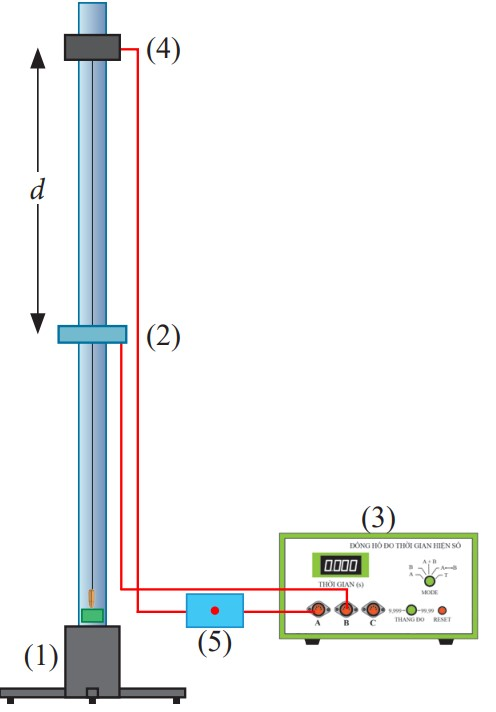
\includegraphics[scale=0.7]{figs/G10-BAI8-1}
		\end{center}
		\textbf{Sơ đồ bố trí thí nghiệm:}\\
		\begin{itemize}[label=$\bullet$]
			\item Giá đỡ (thanh nhôm) có gắn dây dọi (1);
			\item Cổng quang điện (2);
			\item Đồng hồ đo thời gian hiện số (3);
			\item Nam châm điện (4);
			\item Công tắc điện (5);
			\item Vật nặng;
			\item Eke vuông ba chiều dùng để xác định vị trí đầu của vật rơi;
			\item Thước đo có độ chính xác đến $\si{\milli\meter}$.
		\end{itemize}
	\end{itemize}
	GV quan sát, hỗ trợ các nhóm trong quá trình thực hiện thí nghiệm.\\
	\textit{\underline{* HS thực hiện nhiệm vụ học tập}}\\
	HS tiến hành thí nghiệm nghiêm túc, trật tự, an toàn theo nhóm được phân công.\\
	\textit{\underline{* HS báo cáo kết quả nhiệm vụ học tập}}\\
	Các nhóm HS ghi nhận kết quả đo vào bảng số liệu trong phiếu học tập.
	
}
% ==========================================================================================
\hoatdong
{Xử lí kết quả thí nghiệm và viết bài thu hoạch.
}
{HS xử lí được kết quả thí nghiệm và trình bày được báo cáo thu hoạch sau thí nghiệm.	
}
{Phiếu báo cáo kết quả thí nghiệm của các nhóm HS	
}
{\textit{\underline{* GV chuyển giao nhiệm vụ học tập}}\\
	GV hướng dẫn lại cho HS các bước xử lí kết quả thí nghiệm.\\
	GV yêu cầu các nhóm HS hoàn thành bài thu hoạch tại nhà và nộp lại cho GV vào tiết học tiếp theo.\\
	\textit{\underline{* HS thực hiện nhiệm vụ học tập}}\\
	HS tích lắng nghe, đặt câu hỏi (nếu có).\\
	Các nhóm HS hoàn thành phiếu báo cáo kết quả thí nghiệm tại nhà.\\
	\textit{\underline{* HS báo cáo kết quả nhiệm vụ học tập}}\\
	Các nhóm HS nộp lại phiếu báo cáo cho GV.\\
	GV nhận xét, rút kinh nghiệm cho từng nhóm HS.
}
\section{HỒ SƠ DẠY HỌC}
\subsection{Phiếu báo cáo kết quả thực hành}\newpage
\titlespacing*{\subsection}
{0pt}{0.25\baselineskip}{0.5\baselineskip}
\titlespacing*{\section}
{0pt}{0.25\baselineskip}{0.5\baselineskip}
\begin{center}
	\textbf{BÁO CÁO KẾT QUẢ THỰC HÀNH THÍ NGHIỆM}\\
	\textbf{Bài 8. THỰC HÀNH ĐO GIA TỐC RƠI TỰ DO.}\\
\end{center}
\begin{center}
	\begin{tabular}{L{8cm}L{8cm}}
		Lớp: \dotfill&Nhóm: \dotfill
	\end{tabular}
\end{center}
\begin{center}
	\begin{tabular}{|M{1.25cm}|M{7cm}||M{1.25cm}|M{7cm}|}
		\hline
		\multicolumn{4}{|M{16cm}|}{\thead{Thành viên nhóm}}\\
		\hline
		\thead{STT}&\thead{Họ và tên}&\thead{STT}&\thead{Họ và tên}\\
		\hline
		1&&5&\\
		\hline
		2&&6&\\
		\hline
		3&&7&\\
		\hline
		4&&8&\\
		\hline
	\end{tabular}
\end{center}
\setcounter{section}{0}
\section{MỤC ĐÍCH THÍ NGHIỆM}
\Pointilles[2]
\section{CƠ SỞ LÍ THUYẾT}
\textit{\textbf{\underline{Câu hỏi gợi ý:}}}\\
\begin{enumerate}[label=\bfseries Câu \arabic*., leftmargin=2cm, topsep=0pt]
	\item Thế nào là sự rơi tự do? 
	\item Nêu các đặc điểm của chuyển động rơi tự do \textit{(phương chiều chuyển động, tính chất chuyển động)}.
	\item Gia tốc rơi tự do phụ thuộc các yếu tố nào?
	\item Trong phần giới thiệu của SGK bài 8 trang 48, để đo gia tốc rơi tự do cần phải xác định các đại lượng nào?
	\item Sai số phép đo gia tốc rơi tự do theo tiến trình thí nghiệm SGK bài 8 trang 48 được xác định như thế nào?
\end{enumerate}
\Pointilles[20]
\section{TIẾN HÀNH THÍ NGHIỆM}
\textit{Em hãy trình bày các bước tiến hành thí nghiệm}\\
\Pointilles[27]
\section{KẾT QUẢ THÍ NGHIỆM}
\textit{* Quy ước: 
	\begin{itemize}[topsep=0pt]
		\item Giá trị trung bình của các đại lượng đo trực tiếp được lấy lớn hơn 1 bậc thập phân so với giá trị đo.
		\item Kết quả phép đo gia tốc rơi tự do làm tròn đến 2 chữ số sau dấu phẩy thập phân.
\end{itemize}}
\subsection{THÍ NGHIỆM LẦN 1}
\begin{center}
	\begin{tabular}{|M{1.8cm}|M{1.8cm}|M{1.8cm}|M{1.8cm}|M{1.8cm}|M{3cm}|M{4cm}|}
		\hline
		\multicolumn{7}{|M{16cm}|}{\thead{Bảng kết quả đo thời gian rơi lần 1}}\\
		\multicolumn{7}{|M{16cm}|}{Độ dịch chuyển của vật: $d=$\hspace{1cm}$\pm$\hspace{1cm}$\si{\centi\meter}$}\\
		\hline
		\multicolumn{5}{|M{9cm}|}{\thead{Thời gian rơi\\ $\xsi{t}{\left(\second\right)}$}}& \multirow{2}{*}{\thead{Thời gian rơi\\ trung bình\\ $\xsi{\overline{t}}{\left(\second\right)}$}} & \multirow{2}{*}{\thead{Sai số\\thời gian rơi\\ $\xsi{\Delta t}{\left(\second\right)}=\overline{\Delta t}+\Delta t_{\mathrm{dc}}$}}\\
		\cline{1-5}
		\thead{Lần 1}&\thead{Lần 2}&\thead{Lần 3}&\thead{Lần 4}&\thead{Lần 5}&&\\
		\hline
		&&&&&&\\[20pt]
		\hline
	\end{tabular}
\end{center}
Gia tốc rơi tự do trung bình: $\overline{g}=$ \dotfill\\
Sai số của phép đo gia tốc rơi tự do: $\Delta g=$ \dotfill\\
\Pointilles[2]
Kết quả phép đo gia tốc rơi tự do: $g=\overline{g}\pm\Delta g=$ \dotfill\\
\subsection{THÍ NGHIỆM LẦN 2}
\begin{center}
	\begin{tabular}{|M{1.8cm}|M{1.8cm}|M{1.8cm}|M{1.8cm}|M{1.8cm}|M{3cm}|M{4cm}|}
		\hline
		\multicolumn{7}{|M{16cm}|}{\thead{Bảng kết quả đo thời gian rơi lần 2}}\\
		\multicolumn{7}{|M{16cm}|}{Độ dịch chuyển của vật: $d=$\hspace{1cm}$\pm$\hspace{1cm}$\si{\centi\meter}$}\\
		\hline
		\multicolumn{5}{|M{9cm}|}{\thead{Thời gian rơi\\ $\xsi{t}{\left(\second\right)}$}}& \multirow{2}{*}{\thead{Thời gian rơi\\ trung bình\\ $\xsi{\overline{t}}{\left(\second\right)}$}} & \multirow{2}{*}{\thead{Sai số\\thời gian rơi\\ $\xsi{\Delta t}{\left(\second\right)}=\overline{\Delta t}+\Delta t_{\mathrm{dc}}$}}\\
		\cline{1-5}
		\thead{Lần 1}&\thead{Lần 2}&\thead{Lần 3}&\thead{Lần 4}&\thead{Lần 5}&&\\
		\hline
		&&&&&&\\[20pt]
		\hline
	\end{tabular}
\end{center}
Gia tốc rơi tự do trung bình: $\overline{g}=$ \dotfill\\
Sai số của phép đo gia tốc rơi tự do: $\Delta g=$ \dotfill\\
\Pointilles[2]
Kết quả phép đo gia tốc rơi tự do: $g=\overline{g}\pm\Delta g=$ \dotfill\\
\subsection{THÍ NGHIỆM LẦN 3}
\begin{center}
	\begin{tabular}{|M{1.8cm}|M{1.8cm}|M{1.8cm}|M{1.8cm}|M{1.8cm}|M{3cm}|M{4cm}|}
		\hline
		\multicolumn{7}{|M{16cm}|}{\thead{Bảng kết quả đo thời gian rơi lần 3}}\\
		\multicolumn{7}{|M{16cm}|}{Độ dịch chuyển của vật: $d=$\hspace{1cm}$\pm$\hspace{1cm}$\si{\centi\meter}$}\\
		\hline
		\multicolumn{5}{|M{9cm}|}{\thead{Thời gian rơi\\ $\xsi{t}{\left(\second\right)}$}}& \multirow{2}{*}{\thead{Thời gian rơi\\ trung bình\\ $\xsi{\overline{t}}{\left(\second\right)}$}} & \multirow{2}{*}{\thead{Sai số\\thời gian rơi\\ $\xsi{\Delta t}{\left(\second\right)}=\overline{\Delta t}+\Delta t_{\mathrm{dc}}$}}\\
		\cline{1-5}
		\thead{Lần 1}&\thead{Lần 2}&\thead{Lần 3}&\thead{Lần 4}&\thead{Lần 5}&&\\
		\hline
		&&&&&&\\[20pt]
		\hline
	\end{tabular}
\end{center}
Gia tốc rơi tự do trung bình: $\overline{g}=$ \dotfill\\
Sai số của phép đo gia tốc rơi tự do: $\Delta g=$ \dotfill\\
\Pointilles[2]
Kết quả phép đo gia tốc rơi tự do: $g=\overline{g}\pm\Delta g=$ \dotfill\\
\section{KẾT LUẬN VÀ NHẬN XÉT}
\textit{Học sinh tự kết luận về độ chính xác của kết quả phép đo trong bài thực hành, nhận xét quá trình làm thí nghiệm (những khó khăn đã gặp phải, nguyên nhân gây sai số, biện pháp khắc phục nguyên nhân gây sai số), nhận xét về kết quả làm việc nhóm (ưu điểm và nhược điểm của nhóm).}\\
\Pointilles[18]
\setcounter{subsection}{1}
\subsection{Rubric đánh giá kết quả thực hành}
\begin{center}
	\textbf{TIÊU CHÍ ĐÁNH GIÁ THỰC HÀNH THÍ NGHIỆM}\\
	\textbf{Bài 8. THỰC HÀNH ĐO GIA TỐC RƠI TỰ DO.}
\end{center}
\begin{center}
	\begin{tabular}{L{8cm}L{8cm}}
		Lớp: \dotfill&Nhóm: \dotfill
	\end{tabular}
\end{center}
\begin{center}
	\begin{tabular}{|M{1.25cm}|M{7cm}||M{1.25cm}|M{7cm}|}
		\hline
		\multicolumn{4}{M{16cm}}{\thead{Thành viên nhóm}}\\
		\hline
		\thead{STT}&\thead{Họ và tên}&\thead{STT}&\thead{Họ và tên}\\
		\hline
		1&&5&\\
		\hline
		2&&6&\\
		\hline
		3&&7&\\
		\hline
		4&&8&\\
		\hline
	\end{tabular}
\end{center}
\textit{* Quy ước đánh giá: Ứng với mỗi chỉ số hành vi có 4 mức đánh giá, biểu hiện năng lực tốt nhất được đánh giá ở mức 3.}
\begin{center}
	\begin{longtable}{|M{1.5cm}|M{2cm}|M{1.5cm}|L{9cm}|M{1.25cm}|M{0.75cm}|}
		\hline
		\thead{Thành\\ tố}& \thead{Chỉ số\\ hành vi} &\multicolumn{2}{|M{10.5cm}|}{\thead{Tiêu chí chất lượng}}&\multicolumn{2}{|M{2.5cm}|}{\thead{Điểm}}\\
		\hline
		\multirow{12}{1.5cm}{Lập kế hoạch thí nghiệm} & \multirow{4}{2cm}{Xác định mục tiêu, cơ sở lý thuyết}  & Mức 3 & Xác định rõ ràng, chính xác, logic, nhanh chóng, không cần GV giúp đỡ. & 1.00&$\Box$\\ \cline{3-6}
		
		&  & Mức 2 & Xác định được nhưng có vài lỗi nhỏ, cần sự giúp đỡ của GV để điều chỉnh. & 0.75&$\Box$\\ \cline{3-6}
		
		&  & Mức 1 & Xác định được mục tiêu nhưng không xác định được cơ sở lý thuyết, cần hướng dẫn của GV.  & 0.50&$\Box$\\ \cline{3-6}
		
		&  & Mức 0 & Không xác định được, cần sự chỉ dẫn cụ thể của GV mới làm được.  & 0.00&$\Box$\\
		\cline{2-6}
		& \multirow{4}{2cm}{Đề xuất phương án thí nghiệm}  & Mức 3 & Đề xuất được phương án tối ưu một cách nhanh chóng, không cần sự hỗ trợ của GV.  & 0.75&$\Box$\\ \cline{3-6}
		
		&  & Mức 2 & Đề xuất được phương án có tính khả thi nhưng chưa tối ưu, cần GV sửa
		chữa, bổ sung thêm.  & 0.50&$\Box$\\ \cline{3-6}
		
		&  & Mức 1 & Đề xuất được phương án nhưng thiếu tính khả thi, cần GV định hướng.  & 0.25&$\Box$\\ \cline{3-6}
		
		&  & Mức 0 & Chưa đề xuất được phương án, cần hướng dẫn cụ thể của GV.   & 0.00&$\Box$\\
		\cline{2-6}
		& \multirow{4}{2cm}{Xây dựng tiến trình thí nghiệm}  & Mức 3 & Xác định được các dụng cụ cần thiết, xây dựng được tiến trình thí nghiệm phù hợp.  & 0.75&$\Box$\\ \cline{3-6}
		
		&  & Mức 2 & Xác định được dụng cụ cần thiết, xây dựng tiến trình dựa trên gợi ý của GV.  & 0.50&$\Box$\\ \cline{3-6}
		
		&  & Mức 1 & Xác định dụng cụ thí nghiệm chưa đầy đủ, xây dựng tiến trình dựa trên gợi ý của GV.   & 0.25&$\Box$\\ \cline{3-6}
		
		&  & Mức 0 & Chưa xác định được dụng cụ và tiến trình thí nghiệm, cần hướng dẫn cụ thể của GV.   & 0.00&$\Box$\\
		\hline
		\multirow{12}{1.5cm}{Tiến hành thí nghiệm, thu thập số liệu} & \multirow{4}{2cm}{Bố trí thí nghiệm}  & Mức 3 & Tự lắp ráp nhanh chóng, chính xác. Bố trí dụng cụ đúng sơ đồ, hợp lý về
		mặt không gian. & 1.00&$\Box$\\ \cline{3-6}
		
		&  & Mức 2 & Tự lắp ráp chính xác theo sơ đồ nhưng còn chậm và cần chỉnh sửa về mặt không gian.  & 0.75&$\Box$\\ \cline{3-6}
		
		&  & Mức 1 & Lắp ráp, bố trí theo hướng dẫn của GV nhưng còn vụng về.   & 0.50&$\Box$\\ \cline{3-6}
		
		&  & Mức 0 & Không tự lắp ráp được, GV phải làm mẫu.   & 0.00&$\Box$\\
		\cline{2-6}
		& \multirow{4}{2cm}{Thao tác thí nghiệm}  & Mức 3 & Tự lựa chọn đúng thang đo, điều chỉnh dụng cụ một cách chính xác, nhanh chóng.   & 1.00&$\Box$\\ \cline{3-6}
		
		&  & Mức 2 & Tự lựa chọn đúng thang đo, điều chỉnh được dụng cụ nhưng còn chậm.   & 0.75&$\Box$\\ \cline{3-6}
		
		&  & Mức 1 & Lựa chọn được thang đo, điều chỉnh được dụng cụ dưới sự hướng dẫn của GV.   & 0.50&$\Box$\\ \cline{3-6}
		
		&  & Mức 0 & Không biết cách thao tác.    & 0.00&$\Box$\\
		\cline{2-6}
		& \multirow{4}{2cm}{Quan sát, đọc và ghi kết quả}  & Mức 3 & Quan sát và đọc, ghi kết quả một cách nhanh chóng, chính xác.   & 1.00&$\Box$\\ \cline{3-6}
		
		&  & Mức 2 &  Quan sát và đọc, ghi được kết quả nhưng còn chậm.   & 0.75&$\Box$\\ \cline{3-6}
		
		&  & Mức 1 & Quan sát và đọc, ghi được kết quả dưới sự hướng dẫn của GV.    & 0.50&$\Box$\\ \cline{3-6}
		
		&  & Mức 0 &  Hoàn toàn quan sát và đọc, ghi kết quả theo thao tác mẫu của GV.    & 0.00&$\Box$\\
		\hline
		\multirow{8}{1.5cm}{Thái độ thực hành} & \multirow{4}{2cm}{An toàn thí nghiệm}  & Mức 3 & Đảm bảo các quy tắc an toàn trong thực hành thí nghiệm, tác phong nghiêm túc, trật tự, có tinh thần tự giác trong học tập. & 0.75&$\Box$\\ \cline{3-6}
		
		&  & Mức 2 & Đảm bảo các quy tắc an toàn trong thực hành thí nghiệm, tác phong nghiêm túc, trật tự.  & 0.50&$\Box$\\ \cline{3-6}
		
		&  & Mức 1 & Đảm bảo các quy tắc an toàn trong thực hành thí nghiệm, tác phong nghiêm túc, còn gây mất trật tự trong quá trình thực hành.   & 0.25&$\Box$\\ \cline{3-6}
		
		&  & Mức 0 & Không tuân thủ các quy tắc an toàn thí nghiệm, gây mất trật tự trong giờ thực hành.   & 0.00&$\Box$\\
		\cline{2-6}
		& \multirow{4}{2cm}{Trách nhiệm và tích cực}  & Mức 3 & Có tinh thần trách nhiệm trong làm việc nhóm, $\SI{100}{\percent}$ thành viên tích cực tham gia thực hành.   & 0.75&$\Box$\\ \cline{3-6}
		
		&  & Mức 2 & Có tinh thần trách nhiệm trong làm việc nhóm, $\SI{75}{\percent}$ thành viên tích cực tham gia thực hành.   & 0.50&$\Box$\\ \cline{3-6}
		
		&  & Mức 1 & Xao lãng trong làm việc nhóm, $\SI{50}{\percent}$ thành viên tích cực tham gia thực hành.   & 0.25&$\Box$\\ \cline{3-6}
		
		&  & Mức 0 & Xao lãng trong làm việc nhóm, dưới $\SI{50}{\percent}$ thành viên tham gia thực hành.    & 0.00&$\Box$\\
		\hline
		\multirow{12}{1.5cm}{Xử lý kết quả thí nghiệm} & \multirow{4}{2cm}{Xử lý kết quả đo trực tiếp và gián tiếp}  & Mức 3 & Sử dụng công thức phù hợp, tính toán nhanh chóng, kết quả chính xác, phù hợp với số liệu thực tiễn.  & 1.25&$\Box$\\ \cline{3-6}
		
		&  & Mức 2 & Sử dụng công thức phù hợp, tính toán còn chậm, kết quả còn một vài sai sót nhỏ, phù hợp với số liệu thực tiễn.   & 1.00&$\Box$\\ \cline{3-6}
		
		&  & Mức 1 & Cần sự hướng dẫn của GV, còn nhầm lẫn trong tính toán, kết quả sai lệch so với số liệu thực tiễn.    & 0.50&$\Box$\\ \cline{3-6}
		
		&  & Mức 0 & Không tính toán được.    & 0.00&$\Box$\\
		\cline{2-6}
		& \multirow{4}{2cm}{Độ tin cậy của kết quả thí nghiệm}  & Mức 3 & Sai số tỉ đối của phép đo dưới $\SI{5}{\percent}$.   & 0.75&$\Box$\\ \cline{3-6}
		
		&  & Mức 2 & Sai số tỉ đối của phép đo dưới $\SI{10}{\percent}$.   & 0.50&$\Box$\\ \cline{3-6}
		
		&  & Mức 1 & Sai số tỉ đối của phép đo dưới $\SI{15}{\percent}$.   & 0.25&$\Box$\\ \cline{3-6}
		
		&  & Mức 0 & Không xác định được sai số tỉ đối hoặc sai số tỉ đối trên $\SI{15}{\percent}$.    & 0.00&$\Box$\\
		\cline{2-6}
		& \multirow{4}{2cm}{Kết luận, nhận xét, đánh giá}  & Mức 3 & Viết đúng kết quả phép đo, nhận xét chính xác quá trình làm thí
		nghiệm, tìm được nguyên nhân gây sai số và đề xuất được biện pháp khắc phục.   & 1.00&$\Box$\\ \cline{3-6}
		
		&  & Mức 2 &  Viết đúng kết quả phép đo, nhận xét chính xác quá trình làm thí nghiệm, tìm được nguyên nhân gây sai số nhưng không đề xuất được biện pháp khắc phục.   & 0.75&$\Box$\\ \cline{3-6}
		
		&  & Mức 1 & Viết sai kết quả đo, nhận xét được quá trình làm thí
		nghiệm nhưng còn sơ sài, thiếu chính xác, không tìm được nguyên nhân gây sai số.    & 0.50&$\Box$\\ \cline{3-6}
		
		&  & Mức 0 &  Không có hoặc không thể kết luận, nhận xét.    & 0.00&$\Box$\\
		\hline
		\hline
		\multicolumn{6}{|M{16cm}|}{\thead{TỔNG ĐIỂM: \hspace{1cm} /10.00  }}\\
		\hline
		\hline
	\end{longtable}
\end{center}

